\documentclass[12pt,letterpaper]{article}
\usepackage[T1]{fontenc}
\usepackage[utf8]{inputenc}
\usepackage{newtxtext,newtxmath}
\usepackage{amsmath,amssymb,amsthm,mathtools}
\usepackage[letterpaper,margin=1in]{geometry}
\usepackage{microtype}
\usepackage{enumitem}
\usepackage{booktabs}
\usepackage{tikz}
\usepackage{array}
\usepackage{longtable}
\usepackage[hidelinks]{hyperref}
\allowdisplaybreaks[2]
\setlength{\parindent}{0pt}
\setlength{\parskip}{0.55em}
\renewcommand{\arraystretch}{1.25}

\newtheorem{theorem}{Theorem}[section]
\newtheorem{lemma}[theorem]{Lemma}
\newtheorem{proposition}[theorem]{Proposition}
\newtheorem{corollary}[theorem]{Corollary}
\theoremstyle{definition}
\newtheorem{definition}[theorem]{Definition}
\newtheorem{problem}[theorem]{Open problem}
\theoremstyle{remark}
\newtheorem{remark}[theorem]{Remark}
\newtheorem{example}[theorem]{Example}

\newcommand{\Li}{\operatorname{Li}}
\newcommand{\Log}{\operatorname{Log}}
\newcommand{\Ree}{\operatorname{Re}}
\newcommand{\dd}{\,\mathrm{d}}
\newcommand{\CC}{\mathbb{C}}
\newcommand{\RR}{\mathbb{R}}
\newcommand{\NN}{\mathbb{N}}
\newcommand{\eps}{\varepsilon}
\newcommand{\Dk}{\mathcal{D}_k}
\newcommand{\spn}{\operatorname{span}}
\newcommand{\kerop}{\operatorname{ker}}
\newcommand{\ord}{\operatorname{ord}}
\newcommand{\yD}{\vartheta}
\newcommand{\tagN}{\textup{[new]}}

\title{Zeta Functions and Their Associated Operators\\[0.3em]
\large Draft 3: Corrected and expanded version\thanks{Original 1981 Georgia Institute of Technology manuscript. Earlier corrected editions were prepared with assistance from ChatGPT (OpenAI) and Claude (Anthropic). For provenance, see the acknowledgments and revision log.}}
\author{David Joyner\\[0.2em]\normalsize\texttt{wdjoyner@gmail.com}}
\date{Original draft: 1981\\Corrected and expanded draft: November 2026}

\begin{document}
\maketitle

\begin{abstract}
This edition was revised with AI assistance; the roles and limitations are recorded in the Acknowledgments and revision log.
This edition revisits the 1981 manuscript \emph{Zeta Functions and their
Associated Operators}. It keeps the three themes of the original. These are
random generalized zeta functions, comparison of Euler products, and
operators whose kernels detect zeros of $\zeta(s)$. We place everything in
the framework of Beurling generalized primes. We prove one comparison
principle and derive the original Theorems~2 and~3 from it. We show that
the Euler product over $u_n=\Li^{-1}(n)$ has no zeros in the slit half-plane
$\{\Ree s>0\}\setminus(0,1/2]$. We give a two-line reason why the block
operators of the original have far too many eigenvalues. Every
$\lambda\notin[0,\infty)$ is an eigenvalue. We replace the original
Theorems~5 and~6 by honest statements about multiplier operators. Finally,
we give a formulation that does not need the parameter $\beta$. Two
dilation-sum operators have a joint kernel. The dilation generator acts on
that kernel, and its eigenvalues are exactly the nontrivial zeros of
$\zeta$ in a half-plane. The elementary graph-theoretic connections added here also use only mathematics available by 1981.
\end{abstract}

\tableofcontents

\section{Introduction}\label{sec:introduction}
This corrected edition retains the three themes of the 1981
manuscript: generalized prime systems, comparison of Euler
products, and summation operators that detect zeros of the
Riemann zeta function. The principal results are the comparison
principle, the zero-free extension for the logarithmic-integral
prime model, and a joint-kernel theorem for two dilation sums.
The original block operators have many extraneous eigenvalues.
Their complete spectra cannot be identified with the zeta zeros.

Section~\ref{sec:graphs} supplies elementary directed-graph
interpretations. For a running example, moving every prime
to its successor yields a telescoping comparison:
\begin{equation}\label{eq:intro-telescope}
 \prod_{n\ge1}\frac{1-p_n^{-s}}{1-p_{n+1}^{-s}}
 =1-2^{-s}\qquad (\Ree s>0).
\end{equation}
This is explained by the boundary of a flow on a prime path.

\section{Literature review}\label{sec:literature}
\subsection*{Work through 1981}
Beurling~\cite{Be37} introduced generalized prime systems.
Wintner~\cite{Wi44} studied arithmetic semigroups, and
Bateman and Diamond~\cite{BD69} surveyed their asymptotic theory.
Grosswald and Schnitzer~\cite{GS78} studied zero-preserving
perturbations of Euler products. Hawkins~\cite{Ha58},
Kosambi~\cite{Ko59}, Wunderlich~\cite{Wu74}, and
Heyde~\cite{He78} supplied related random-prime models.

In operator theory, Schwartz~\cite{Sc47} developed spectral
synthesis for mean-periodic functions. Nyman~\cite{Ny50}
and Beurling~\cite{Be55} examined closure questions related
to the zeta function. No unproved spectral-synthesis
conclusion is borrowed from these works.

\subsection*{Later work}
This historical edition does not invoke results obtained
after 1981. Modern operator models and modern graph-zeta
theory belong in separate contemporary manuscripts.

\section{Background and classical input}\label{sec:background}

\subsection{Beurling generalized primes}

A \emph{Beurling generalized prime system} is a sequence $A=(a_n)$ of real
numbers with $1<a_1\le a_2\le\cdots$ and $a_n\to\infty$. This framework is
due to Beurling~\cite{Be37}. Wintner~\cite{Wi44} studied related
arithmetical semigroups. Bateman and Diamond~\cite{BD69} surveyed the
theory in 1969. The \emph{generalized integers} are the formal finite products
of the $a_n$. They are counted with multiplicity. Two products with
different exponent vectors count as different integers, even if their
numerical values agree.

With this convention we have the formal identity
\[
\zeta_A(s)=\sum_{\nu}\nu^{-s}=\prod_{n\ge1}(1-a_n^{-s})^{-1},
\]
where $\nu$ runs over the generalized integers with multiplicity. For example, if $a_1=a_2=3$, three different exponent vectors give the
numerical value $9$, and all three must be counted.
Both sides converge absolutely when $\sum_n a_n^{-\sigma}<\infty$. Every system
in this paper has $a_n\asymp n\log n$. So both sides converge for
$\Ree s>1$.

\begin{remark}\label{rem:UF}
Unique factorization of the \emph{numbers} $a_n$ plays no role in the
Euler product. It matters only if one wants the Dirichlet series to run
over distinct real numbers. The typescript spends effort on unique
factorization in Lemma~1(c) and Theorem~3. In the Beurling framework that
effort is unnecessary.
\end{remark}

\subsection{The logarithmic integral}

On $(1,\infty)$ the function $\Li$ is smooth and strictly increasing. It
tends to $-\infty$ as $x\to1^+$ and to $+\infty$ as $x\to\infty$. So
$\Li^{-1}$ maps $\RR$ onto $(1,\infty)$. Its unique zero $\mu$ satisfies
$1<\mu<2$. We have $\Li(x)\sim x/\log x$ and $u_n=\Li^{-1}(n)\sim n\log n$.
Also $u_1>\mu$.

\subsection{Classical input}

We use the following facts. All were known in 1981. Standard references
are Ingham~\cite{In32} and Titchmarsh~\cite{Ti51}.
\begin{enumerate}[label=(C\arabic*),leftmargin=3em]
\item\label{C:pnt} The prime number theorem in the form
  $\pi(x)\sim\Li(x)$. So $p_n\sim n\log n$. Also $p_{n+1}<2p_n$
  (Bertrand's postulate).
\item\label{C:ingham} For each $\delta>0$,
  $\pi(x)-\Li(x)\ll_\delta x^{\theta+\delta}$. This follows from the
  explicit formula. See Ingham~\cite{In32}.
\item\label{C:koch} If the Riemann hypothesis holds, then
  $\pi(x)-\Li(x)\ll\sqrt{x}\log x$. This is due to von
  Koch~\cite{vK01}.
\item\label{C:hoeffding} Hoeffding's inequality~\cite{Ho63}. Let
  $Y_1,\dots,Y_n$ be independent with values in $[-1,1]$ and mean $0$.
  Then $\Pr(|Y_1+\cdots+Y_n|>t)\le 2\exp(-t^2/(2n))$.
\item\label{C:BC} The Borel--Cantelli lemma.
\item\label{C:E1} The exponential integral. For $\Ree w>0$ and $a>0$,
  \[
  \int_a^\infty e^{-wv}\frac{\dd v}{v}
  =-\gamma-\Log(aw)-\sum_{j\ge1}\frac{(-aw)^j}{j\cdot j!}.
  \]
  Here $\gamma$ is Euler's constant. The series is entire in $w$.
\item\label{C:eta} The series $\eta(s)=\sum(-1)^{n-1}n^{-s}$ converges
  for $\Ree s>0$, locally uniformly. Its termwise derivatives also
  converge. The factor $1-2^{1-s}$ vanishes only on the line $\Ree s=1$.
  It vanishes there exactly at $s=1+2\pi i m/\log2$ with $m\in\mathbb Z$.
  Also $\eta(1)=\log 2\ne0$, and $\eta(x)>0$ for $0<x<1$.
\end{enumerate}

\begin{lemma}\label{lem:pnun}
For every $\delta>0$ we have $|p_n-u_n|\ll_\delta n^{\theta+\delta}$. If
the Riemann hypothesis holds, then $|p_n-u_n|\ll n^{1/2}(\log n)^{5/2}$.
\end{lemma}

\begin{proof}
By the mean value theorem,
$\Li(p_n)-\Li(u_n)=(p_n-u_n)/\log\xi_n$ for some $\xi_n$ between $p_n$
and $u_n$. Here $\Li(u_n)=n=\pi(p_n)$. So
\[
|p_n-u_n|=\log\xi_n\cdot|\Li(p_n)-\pi(p_n)|.
\]
Both $p_n$ and $u_n$ are $\asymp n\log n$. So $\log\xi_n\ll\log n$. Now
apply \ref{C:ingham}, or \ref{C:koch} under RH. When $\theta=1$ the first
bound also follows from $p_n,u_n\ll n\log n$.
\end{proof}

\section{Notation}\label{sec:notation}

\begin{longtable}{@{}p{0.24\textwidth}p{0.7\textwidth}@{}}
\toprule
\textbf{Symbol} & \textbf{Meaning}\\
\midrule
\endhead
$s=\sigma+it$ & A complex variable with $\sigma=\Ree s$.\\
$p_n$ & The $n$th rational prime.\\
$\pi(x)$ & The number of primes $p\le x$.\\
$\Li(x)$ & The logarithmic integral $\mathrm{P.V.}\int_0^x \dd t/\log t$ for
$x>1$.\\
$\mu$ & The unique zero of $\Li$ in $(1,\infty)$. Numerically
$\mu\approx 1.4513$.\\
$u_n$ & $\Li^{-1}(n)$ for $n\ge1$. So $u_n\sim n\log n$.\\
$A=(a_n)$ & A Beurling generalized prime system, $1<a_1\le a_2\le\cdots$,
$a_n\to\infty$.\\
$\pi_A(x)$ & The number of $n$ with $a_n\le x$.\\
$\zeta_A(s)$ & The Euler product $\prod_n(1-a_n^{-s})^{-1}$.\\
$\zeta_U,\ \zeta_G$ & $\zeta_A$ for $a_n=u_n$, and for the random system
$a_n=g_n$ of Section~\ref{sec:random}.\\
$P_A(s)$ & The prime zeta function $\sum_n a_n^{-s}$.\\
$\Theta_A,\ \Psi_A$ & Chebyshev functions $\sum_{a_n\le x}\log a_n$ and
$\sum_{m\ge1}\Theta_A(x^{1/m})$.\\
$\eta(s)$ & The Dirichlet eta function
$\sum_{n\ge1}(-1)^{n-1}n^{-s}=(1-2^{1-s})\zeta(s)$.\\
$\theta$ & $\sup\{\Ree\rho:\zeta(\rho)=0,\ 0<\Ree\rho<1\}$. So
$\tfrac12\le\theta\le1$.\\
$\ord_\rho F$ & The order of vanishing of a holomorphic $F$ at $\rho$.\\
$\Log$ & The principal branch of the logarithm on
$\CC\setminus(-\infty,0]$.\\
$k,\ \alpha$ & A positive integer, and $\alpha=1/(2k)$.\\
$S_k$ & The weighted Sobolev space of Section~\ref{sec:operators}.\\
$\|\cdot\|_k$ & Its norm.\\
$D$ & Differentiation $\dd/\dd y$ in the distributional sense.\\
$\yD$ & The dilation generator $yD$, so $\yD f(y)=yf'(y)$.\\
$\Dk$ & The span of $y^s(\log y)^j$ with $\Ree s>\alpha$ and $j\ge0$.\\
$R_c$ & Dilation, $(R_cf)(y)=f(y/c)$ for $c>1$.\\
$J_\beta$ & The Euler operator $y^2D^2+(1-2\beta)yD=\yD(\yD-2\beta)$.\\
$T$ & The alternating dilation sum $\sum_{n\ge1}(-1)^nR_n$.\\
$T^{(q)}$ & The dilation sum with symbol $(1-q^{1-s})\zeta(s)$. Note
$T=-T^{(2)}$.\\
$M$ & Multiplication by $-\log y$.\\
$B(\beta)$ & The block operator $\begin{psmallmatrix}J_\beta&0\\
T&M\end{psmallmatrix}$ on $S_k\oplus S_k$.\\
$F(\Delta)$ & The multiplier operator on $\Dk$ with symbol $F$
(Definition~\ref{def:multiplier}).\\
$f\ll g$ & $|f|\le Cg$ for a constant $C$. A subscript shows what $C$
depends on.\\
\bottomrule
\end{longtable}


\section{A comparison principle for Euler products}\label{sec:comparison}

This section replaces the double series of the typescript. We compare
Euler factors directly. The method goes back to Grosswald and
Schnitzer~\cite{GS78}.

\begin{lemma}[Factor bound]\label{lem:factor}
Let $a,b>1$ and let $m=\min(a,b)$. Let $\Ree s=\sigma>0$ with
$m^{-\sigma}\le\frac12$. Define $\log(1-z)=-\sum_{j\ge1}z^j/j$ for
$|z|<1$. Then
\[
\bigl|\log(1-a^{-s})-\log(1-b^{-s})\bigr|\le 2|s|\,|a-b|\,m^{-1-\sigma}.
\]
\end{lemma}

\begin{proof}
For $c>1$ the derivative in $c$ is
\[
\frac{\partial}{\partial c}\log(1-c^{-s})=\frac{s\,c^{-s-1}}{1-c^{-s}}.
\]
For $c\ge m$ the denominator has modulus at least $1-m^{-\sigma}\ge\frac12$.
So the derivative has modulus at most $2|s|c^{-1-\sigma}\le2|s|m^{-1-\sigma}$.
Integrate over the real segment from $a$ to $b$.
\end{proof}

\begin{theorem}[Comparison principle, new]\label{thm:comparison}
Let $A=(a_n)$ and $B=(b_n)$ be sequences with $a_n,b_n>1$. Put
$m_n=\min(a_n,b_n)$ and assume $m_n\to\infty$. Let $\sigma_0\ge0$. Assume
that
\begin{equation}\label{eq:l1}
\sum_{n\ge1}|a_n-b_n|\,m_n^{-1-\sigma}<\infty
\qquad\text{for every }\sigma>\sigma_0.
\end{equation}
Then the product
\[
Q(s)=\prod_{n\ge1}\frac{1-b_n^{-s}}{1-a_n^{-s}}
\]
converges normally on compact subsets of $\Ree s>\sigma_0$. Its limit is
holomorphic and has no zeros there. Where both Euler products converge we
have $Q=\zeta_A/\zeta_B$. In particular, if $\zeta_B$ continues
meromorphically to $\Ree s>\sigma_0$, then so does $\zeta_A=Q\zeta_B$. The
two functions then have the same zeros and poles there, with
multiplicities.
\end{theorem}

\begin{proof}
Let $K$ be a compact subset of $\Ree s>\sigma_0$. Put
$\sigma_K=\min_K\Ree s$. Choose $n_K$ such that $m_n^{-\sigma_K}\le\frac12$
for $n\ge n_K$. Write
$\ell_n(s)=\log(1-b_n^{-s})-\log(1-a_n^{-s})$. Each $\ell_n$ is
holomorphic on $\Ree s>0$, since $|a_n^{-s}|,|b_n^{-s}|<1$ there. For
$n\ge n_K$ and $s\in K$, Lemma~\ref{lem:factor} gives
\[
|\ell_n(s)|\le 2\max_K|s|\cdot|a_n-b_n|\,m_n^{-1-\sigma_K}.
\]
By \eqref{eq:l1} with $\sigma=\sigma_K$ the series $\sum\ell_n$ converges
uniformly on $K$. Its sum $L$ is holomorphic, and $Q=e^L$ has no zeros.
\end{proof}

The hypothesis \eqref{eq:l1} is a weighted $\ell^1$ condition. It allows
large individual errors, provided they are rare. The next lemma turns
counting information into \eqref{eq:l1}.

\begin{lemma}[Dyadic counting, new]\label{lem:dyadic}
Let $w_n\ge0$. Let $0\le\kappa\le1$, $\tau\ge0$ and $\sigma_0\ge0$.
Assume:
\begin{enumerate}[label=(\roman*)]
\item $w_n\ll_\delta n^{\kappa+\delta}$ for every $\delta>0$.
\item For every sufficiently small $\eps>0$, the count
  $E_\eps(t)=\#\{n\le t:\ w_n\ge n^{\tau+\eps}\}$ satisfies
  $E_\eps(t)\ll_\eps t^{1+\sigma_0-\kappa+\eps}$.
\end{enumerate}
Then $\sum_n w_n n^{-1-\sigma}<\infty$ for every
$\sigma>\max(\tau,\sigma_0)$.
\end{lemma}

\begin{proof}
Fix $\sigma>\max(\tau,\sigma_0)$. Choose small $\eps,\delta>0$ with
$\sigma>\tau+\eps$, $\sigma>\sigma_0+\eps+\delta$ and $\delta<\sigma$.
Call $n$ \emph{good} if $w_n<n^{\tau+\eps}$. Otherwise call $n$
\emph{exceptional}. The good terms are at most $n^{\tau+\eps-1-\sigma}$.
Their sum converges because $\sigma>\tau+\eps$.

For the exceptional terms use (i). The exponent $\kappa+\delta-1-\sigma$
is negative. So on the block $2^j\le n<2^{j+1}$ each exceptional term is
$\ll 2^{j(\kappa+\delta-1-\sigma)}$. The block has at most
$E_\eps(2^{j+1})$ exceptional terms. By (ii) its total is
\[
\ll 2^{j(\kappa+\delta-1-\sigma)}\cdot2^{j(1+\sigma_0-\kappa+\eps)}
=2^{-j(\sigma-\sigma_0-\eps-\delta)}.
\]
This is summable over $j$.
\end{proof}

We now recover three statements as corollaries.

\begin{corollary}[After Grosswald and Schnitzer]\label{cor:GS}
Let $q_n$ be real numbers with $p_n\le q_n\le p_{n+1}$. Then $\zeta_Q/\zeta$
extends to a holomorphic function without zeros on $\Ree s>0$. So
$\zeta_Q$ and $\zeta$ have the same zeros in $\Ree s>0$, with
multiplicities.
\end{corollary}

\begin{proof}
Here $m_n=p_n$ and $|q_n-p_n|\le p_{n+1}-p_n$. By \ref{C:pnt},
$p_{n+1}<2p_n$. So for $x\in[p_n,p_{n+1}]$ we have
$p_n^{-1-\sigma}\le2^{1+\sigma}x^{-1-\sigma}$. Hence
\[
\sum_n(p_{n+1}-p_n)p_n^{-1-\sigma}
\le2^{1+\sigma}\int_2^\infty x^{-1-\sigma}\dd x<\infty
\]
for every $\sigma>0$. Apply Theorem~\ref{thm:comparison} with
$\sigma_0=0$.
\end{proof}

\begin{remark}
Grosswald and Schnitzer~\cite{GS78} proved a result of this type in 1978.
The typescript cites their paper for its ``method of analytic
continuation.'' The proof above shows that no bound on individual prime
gaps is needed. Only the average size of the gaps enters.
\end{remark}

\begin{corollary}[Original Corollary 1, repaired]\label{cor:pointwise}
Let $0\le\vartheta<1$. Let $a_n>1$ with $|a_n-p_n|\ll_\delta
n^{\vartheta+\delta}$ for every $\delta>0$. Then $\zeta_A$ and $\zeta$
have the same zeros and poles in $\Ree s>\vartheta$, with multiplicities.
The case $\vartheta=1/(2k)$ is the original Corollary~1.
\end{corollary}

\begin{proof}
Since $\vartheta<1$, we have $a_n=p_n+o(n)$. So $m_n\gg n\log n\ge n$. The
series in \eqref{eq:l1} is $\ll\sum_n n^{\vartheta+\delta-1-\sigma}$. It
converges for $\sigma>\vartheta+\delta$. Since $\delta$ is arbitrary,
\eqref{eq:l1} holds with $\sigma_0=\vartheta$.
\end{proof}

\begin{corollary}[Original Theorem 3, repaired]\label{cor:sparseA}
Let $0\le\vartheta<1$ and $\sigma_0>0$. Let $a_n>1$. Assume:
\begin{enumerate}[label=(\roman*)]
\item $|a_n-p_n|\ll_\delta n^{\vartheta+\delta}$ for every $\delta>0$.
\item For every sufficiently small $\eps>0$,
\[
\#\{n:\ p_n\le X,\ |a_n-p_n|\ge n^{\sigma_0+\eps}\}
\ll_\eps X^{1+\sigma_0-\vartheta+\eps}.
\]
\end{enumerate}
Then $\zeta_A$ and $\zeta$ have the same zeros and poles in
$\Ree s>\sigma_0$, with multiplicities.
\end{corollary}

\begin{proof}
If $n\le t$ then $p_n\le p_t\le Ct\log t$. So the count in (ii), taken over
$n\le t$, is $\ll_\eps t^{1+\sigma_0-\vartheta+2\eps}$. Apply
Lemma~\ref{lem:dyadic} with $w_n=|a_n-p_n|$, $\kappa=\vartheta$ and
$\tau=\sigma_0$, using $2\eps$ in place of $\eps$. As before
$m_n\gg n$. So \eqref{eq:l1} holds for every $\sigma>\sigma_0$. Apply
Theorem~\ref{thm:comparison}.
\end{proof}

\begin{remark}
The typescript lists $a_1=1$ as a generator. That is impossible. The
factor $(1-1^{-s})^{-1}$ is undefined. The identity element belongs to
the semigroup of generalized integers. It is never a generator.
\end{remark}

\section{The deterministic system \texorpdfstring{$u_n=\Li^{-1}(n)$}{u\_n = Li\^{}(-1)(n)}}
\label{sec:deterministic}

In this section $U=(u_n)$ with $u_n=\Li^{-1}(n)$. Its counting function is
as regular as possible. For $x\ge u_1$ we have $\Li(x)\ge1$, and $u_n\le x$
holds exactly when $n\le\Li(x)$. So
\begin{equation}\label{eq:piU}
\pi_U(x)=\lfloor\Li(x)\rfloor=\Li(x)-\{\Li(x)\}\qquad(x\ge u_1).
\end{equation}
Write $b(x)=\{\Li(x)\}$ for $x\ge u_1$. Then $0\le b(x)<1$ and $b(u_1)=0$.

\begin{lemma}[New]\label{lem:PU}
The prime zeta function $P_U(s)=\sum_n u_n^{-s}$ satisfies
\[
P_U(s)=-\Log(s-1)+H(s)\qquad(\Ree s>1),
\]
where $H$ extends to a holomorphic function on $\Ree s>0$.
\end{lemma}

\begin{proof}
Fix $X>u_1$ and $\Ree s>1$. The sum over $u_n\le X$ is $u_1^{-s}$ plus a
Stieltjes integral over $(u_1,X]$. By \eqref{eq:piU},
\[
\sum_{u_n\le X}u_n^{-s}
=u_1^{-s}+\int_{u_1}^X x^{-s}\frac{\dd x}{\log x}
-\int_{(u_1,X]}x^{-s}\dd b(x).
\]
Integrate the last term by parts. Since $b(u_1)=0$, it equals
$X^{-s}b(X)+s\int_{u_1}^X b(x)x^{-s-1}\dd x$. Let $X\to\infty$. We get
\[
P_U(s)=u_1^{-s}+I(s)-s\int_{u_1}^\infty b(x)x^{-s-1}\dd x,
\qquad I(s)=\int_{u_1}^\infty x^{-s}\frac{\dd x}{\log x}.
\]
The last integral converges absolutely and locally uniformly on $\Ree s>0$,
because $|b|<1$. Substitute $x=e^v$ in $I(s)$. With $a=\log u_1>0$ we get
$I(s)=\int_a^\infty e^{-(s-1)v}\,\dd v/v$. By \ref{C:E1}, $I(s)+\Log(s-1)$
is an entire function of $s$.
\end{proof}

\begin{theorem}[Replaces original Theorem 6, new]\label{thm:slit}
Let $\Omega=\{\Ree s>0\}\setminus(0,\tfrac12]$. Then $\zeta_U$ extends to a
meromorphic function on $\Omega$. Its only singularity is a simple pole at
$s=1$. It has no zeros in $\Omega$. Near $s=\frac12$ we have
\[
\zeta_U(s)=(2s-1)^{-1/2}\,E(s),
\]
where $E$ is holomorphic and nonzero near $\tfrac12$. So $s=\tfrac12$ is a
branch point. In particular $\zeta_U$ is meromorphic on $\Ree s>\tfrac12$
with a simple pole at $1$ and no zeros. It has no meromorphic
continuation to any neighborhood of $\tfrac12$.
\end{theorem}

\begin{proof}
By Lemma~\ref{lem:PU}, $P_U$ extends holomorphically to
$\Omega_1=\{\Ree s>0\}\setminus(0,1]$. For $m\ge2$, the function
$s\mapsto P_U(ms)$ is holomorphic on $\{\Ree s>0\}\setminus(0,1/m]$. This
set contains $\Omega$. Define on $\Omega$
\[
F(s)=H(s)+\sum_{m\ge2}\frac{P_U(ms)}{m}.
\]
We check that the series converges locally uniformly. Let $K\subset\Omega$
be compact and $\sigma_K=\min_K\Ree s>0$. If $m\sigma_K\ge2$, then
$\Ree(ms)\ge2$. There $P_U(ms)$ is given by its series. Since $u_n\ge u_1>1$,
\[
|P_U(ms)|\le\sum_n u_n^{-m\sigma_K}
\le u_1^{2-m\sigma_K}\sum_n u_n^{-2}.
\]
The last sum is finite. So the tail is dominated by a geometric series.
The finitely many other terms are holomorphic on $K$. So $F$ is
holomorphic on $\Omega$.

For $\Ree s>1$ all series converge absolutely. Then
\[
\log\zeta_U(s)=\sum_n\sum_{m\ge1}\frac{u_n^{-ms}}{m}
=\sum_{m\ge1}\frac{P_U(ms)}{m}=-\Log(s-1)+F(s).
\]
So $\zeta_U(s)=e^{F(s)}/(s-1)$ for $\Ree s>1$. The right side is
meromorphic on $\Omega$. Its only pole is at $s=1$, and it has no zeros.

Near $s=\frac12$, every term of $F$ except $m=2$ is holomorphic. The term
$m=2$ is $\tfrac12P_U(2s)=-\tfrac12\Log(2s-1)+\tfrac12H(2s)$. So
$e^{F(s)}=(2s-1)^{-1/2}\exp\bigl(\tfrac12H(2s)+F_2(s)\bigr)$, with $F_2$
holomorphic near $\frac12$. This gives the stated form of $\zeta_U$.
\end{proof}

\begin{remark}
The first corrected edition proved only the half-plane $\Ree s>\frac12$.
It worked with $\Psi_U$, which mixes all prime powers. The term
$\Theta_U(\sqrt{x})\approx\sqrt{x}$ in $\Psi_U$ is the trace of the branch
point at $\frac12$. Working with $P_U$ separates the prime powers. Then
each $m$ contributes one branch point, at $s=1/m$.
\end{remark}

\begin{remark}
Theorem~\ref{thm:slit} needs no unique factorization of the numbers
$u_n$. Whether the $u_n$ are multiplicatively independent is not known to
us. It does not matter here (Remark~\ref{rem:UF}).
\end{remark}

\section{Sparse exceptions for the ordinary primes}\label{sec:sparse}

For $\eps>0$ define
\[
P_\eps(X)=\#\{n:\ p_n\le X,\ |p_n-u_n|\ge n^{1/2+\eps}\}.
\]

\begin{theorem}[Original Theorem 2, repaired]\label{thm:sparse}
Let $\sigma_0\ge\frac12$. Suppose that for every sufficiently small
$\eps>0$,
\begin{equation}\label{eq:sparsehyp}
P_\eps(X)\ll_\eps X^{1+\sigma_0-\theta+\eps}.
\end{equation}
Then $\zeta(s)$ has no zeros in $\Ree s>\sigma_0$. That is,
$\theta\le\sigma_0$.
\end{theorem}

\begin{proof}
Put $w_n=|p_n-u_n|$. By Lemma~\ref{lem:pnun}, condition (i) of
Lemma~\ref{lem:dyadic} holds with $\kappa=\theta$. As in the proof of
Corollary~\ref{cor:sparseA}, \eqref{eq:sparsehyp} gives condition (ii) with
$\tau=\frac12$. So $\sum w_nn^{-1-\sigma}<\infty$ for every
$\sigma>\max(\frac12,\sigma_0)=\sigma_0$.

Both $p_n$ and $u_n$ are $\gg n\log n$. So \eqref{eq:l1} holds for $A=U$
and $B$ the primes. Theorem~\ref{thm:comparison} gives
$\zeta_U=Q\,\zeta$ on $\Ree s>\sigma_0$, with $Q$ holomorphic and never zero.
By Theorem~\ref{thm:slit}, $\zeta_U$ has no zeros in $\Ree s>\frac12$. So
$\zeta=\zeta_U/Q$ has no zeros in $\Ree s>\sigma_0$.
\end{proof}

The hypothesis involves the unknown number $\theta$. Since $\theta\le1$, we
can remove it.

\begin{corollary}[$\theta$-free form, new]\label{cor:thetafree}
Let $\sigma_0\ge\frac12$. Suppose $P_\eps(X)\ll_\eps X^{\sigma_0+\eps}$ for
every sufficiently small $\eps>0$. Then $\zeta(s)$ has no zeros in
$\Ree s>\sigma_0$.
\end{corollary}

\begin{proof}
Since $\theta\le1$, we have $X^{\sigma_0+\eps}\le X^{1+\sigma_0-\theta+\eps}$.
Apply Theorem~\ref{thm:sparse}.
\end{proof}

\begin{corollary}[New]\label{cor:RHequiv}
The following are equivalent.
\begin{enumerate}[label=(\alph*)]
\item The Riemann hypothesis.
\item For every $\eps>0$, only finitely many $n$ satisfy
  $|p_n-u_n|\ge n^{1/2+\eps}$.
\item For every sufficiently small $\eps>0$,
  $P_\eps(X)\ll_\eps X^{1/2+\eps}$.
\end{enumerate}
\end{corollary}

\begin{proof}
Assume (a). Lemma~\ref{lem:pnun} gives $|p_n-u_n|\ll n^{1/2}(\log
n)^{5/2}$. This is less than $n^{1/2+\eps}$ for large $n$. So (b) holds.
Clearly (b) implies (c). Corollary~\ref{cor:thetafree} with
$\sigma_0=\frac12$ shows that (c) implies (a).
\end{proof}

\begin{remark}[Contrapositive form]
Theorem~\ref{thm:sparse} is an oscillation theorem in disguise. Suppose
$\zeta$ has a zero with real part greater than $\sigma_0$. Then for
arbitrarily small $\eps$ the large deviations $|p_n-u_n|\ge n^{1/2+\eps}$
are \emph{not} as rare as $X^{1+\sigma_0-\theta+\eps}$.
\end{remark}

\begin{remark}[Why the last step of the typescript fails]
The typescript estimates $\int_1^N x^a\dd P_\eps(x)\ll P_\eps(N)N^a$ for
$a<0$. This is false in general. Early jumps of $P_\eps$ carry more weight
than late ones. Also, bounded partial sums would not prove the convergence
needed for analytic continuation. Lemma~\ref{lem:dyadic} gives absolute and
locally uniform convergence instead.
\end{remark}

\begin{remark}[A divergence statement, new]
For every $\sigma<\frac12$ we have $\sum_n|p_n-u_n|\,n^{-1-\sigma}=\infty$.
Suppose the series converged for some $\sigma_1<\frac12$. Then
Theorem~\ref{thm:comparison} would give $\zeta=\zeta_U/Q$ on
$\Omega\cap\{\Ree s>\sigma_1\}$. By Theorem~\ref{thm:slit}, $\zeta$ would
have no zeros off the real axis there. But $\zeta$ has zeros on
$\Ree s=\frac12$ off the real axis. This is weaker than Littlewood's
oscillation theorem~\cite{Li14}. It is a pleasant consistency check.
\end{remark}

\section{A random model}\label{sec:random}

This section is logically independent of the rest. Theorem~\ref{thm:sparse}
no longer needs it. Random models of the primes were known in 1981. See
Hawkins~\cite{Ha58}, Wunderlich~\cite{Wu74} and
Heyde~\cite{He78}. Our model randomizes the counting function
$\Li$ directly. It follows a suggestion of Kosambi~\cite{Ko59}.

\begin{theorem}[Original Theorem 1, repaired]\label{thm:random}
Let $X_1,X_2,\dots$ be independent and uniform on $(0,2)$. Put
$S_n=X_1+\cdots+X_n$ and $g_n=\Li^{-1}(S_n)$. Then $1<g_1<g_2<\cdots$.
With probability one the following hold.
\begin{enumerate}[label=(\roman*)]
\item The $g_n$ are multiplicatively independent.
\item $\pi_G(x)=\Li(x)+O_\omega(\sqrt{x})$ as $x\to\infty$.
\item $\zeta_G$ is meromorphic on $\Ree s>\frac12$. Its only pole is a
  simple pole at $s=1$. It has no zeros there.
\end{enumerate}
\end{theorem}

\begin{proof}
\emph{Concentration.} Put $Y_j=X_j-1$. By \ref{C:hoeffding} with
$t=3\sqrt{n\log n}$,
\[
\Pr\bigl(|S_n-n|>3\sqrt{n\log n}\bigr)\le2\exp\Bigl(-\frac{9n\log n}{2n}\Bigr)
=2n^{-9/2}.
\]
This is summable. By \ref{C:BC}, almost surely
$S_n=n+O_\omega(\sqrt{n\log n})$.

\emph{Inversion.} The $S_n$ increase strictly. Let
$N_\omega(t)=\#\{n:\ S_n\le t\}$. Compare $S_n$ with $t$ at
$n=\lfloor t\pm C\sqrt{t\log t}\rfloor$. This gives
$N_\omega(t)=t+O_\omega(\sqrt{t\log t})$. Now $\pi_G(x)=N_\omega(\Li(x))$
and $\Li(x)\asymp x/\log x$. So $\pi_G(x)=\Li(x)+O_\omega(\sqrt{x})$.

\emph{Independence.} Fix a nonzero integer vector $(e_1,\dots,e_m)$ with
$e_m\ne0$. Condition on $X_1,\dots,X_{m-1}$. Then $g_m$ is a continuous,
strictly increasing function of $X_m$. The relation
$\prod_jg_j^{e_j}=1$ determines $g_m$ uniquely. So it holds with
conditional probability zero. There are countably many integer vectors.
So almost surely no relation holds.

\emph{Continuation.} Work on a sample point where (ii) holds. Stieltjes
integration and (ii) give $\Theta_G(x)=x+O_\omega(\sqrt{x}\log x)$. The main
term comes from $\int\log t\dd\Li(t)=\int\dd t$. Every $g_n$ exceeds $\mu>1$.
So only $O(\log x)$ values of $m$ give $\Theta_G(x^{1/m})\ne0$. Each such
term with $m\ge2$ is $\ll\sqrt{x}$. Hence $\Psi_G(x)=x+O_\omega(\sqrt{x}\log
x)$.

For $\Ree s>1$, logarithmic differentiation of the Euler product gives
\[
-\frac{\zeta_G'(s)}{\zeta_G(s)}=s\int_1^\infty\Psi_G(x)x^{-s-1}\dd x.
\]
The coefficient of $g^{-ms}$ here is $\log g$. It is not $(\log g)/m$, as
the typescript has it. The factor $1/m$ belongs to $\log\zeta_G$, before
differentiation. Since $s\int_1^\infty x\cdot x^{-s-1}\dd x=1+1/(s-1)$, we
get
\[
-\frac{\dd}{\dd s}\log\bigl((s-1)\zeta_G(s)\bigr)
=1+s\int_1^\infty(\Psi_G(x)-x)x^{-s-1}\dd x.
\]
The integral converges locally uniformly on $\Ree s>\frac12$. So the right
side is holomorphic there. The half-plane is simply connected. Integrating
gives a holomorphic logarithm of $(s-1)\zeta_G(s)$. So $(s-1)\zeta_G(s)$
continues holomorphically and has no zeros on $\Ree s>\frac12$.
\end{proof}

\begin{remark}
Theorem~\ref{thm:random} is an almost-sure asymptotic statement. It does
not reproduce the finite-$n$ inequalities of Lemma~1 with their constants.
Those constants are not needed. Part~(i) is true but, by
Remark~\ref{rem:UF}, it is not needed for part~(iii).
\end{remark}

\begin{remark}
The typescript observes that consecutive $g_n$ differ by $O(\log g_n)$.
By Rankin's theorem~\cite{Ra38} on large prime gaps, no choice of the
$X_n$ makes $g_n=p_n$ for all $n$. This remark is correct.
\end{remark}

\begin{remark}
The random generators $g_n$ differ from $u_n$ by about
$\sqrt{n}\,(\log n)^{3/2}$. Under RH the primes $p_n$ differ from $u_n$ by
a similar amount (Lemma~\ref{lem:pnun}). So under RH the $g_n$ are, almost
surely, a perturbation of the primes of the kind allowed in
Corollary~\ref{cor:pointwise} with $\vartheta=\frac12$. This only
confirms that both functions are zero-free in $\Ree s>\frac12$.
\end{remark}

\section{Operators on a weighted Sobolev space}\label{sec:operators}

\subsection{The space}

Fix integers $k\ge1$ and $N\ge2$. Put $\alpha=1/(2k)$.
The notation $S_k$ suppresses the fixed order $N$.

\begin{definition}
$S_k$ is the space of functions $f$ on $(0,1)$ whose distributional
derivatives satisfy
\[
\|f\|_k^2=\sum_{j=0}^N\int_0^1|D^jf(y)|^2\,y^{2j-1-1/k}\dd y<\infty.
\]
\end{definition}

\begin{lemma}\label{lem:powers}
For complex $s$ and $j\ge0$, the function $y^s(\log y)^j$ lies in $S_k$
if and only if $\Ree s>\alpha$.
\end{lemma}

\begin{proof}
The $i$th derivative of $y^s(\log y)^j$ is $y^{s-i}$ times a polynomial
in $\log y$. With the weight, the $i$th integrand is
$y^{2\Ree s-1-1/k}$ times a power of $|\log y|$. Near $y=0$ this is
integrable exactly when $2\Ree s>1/k$. Near $y=1$ there is no problem.
\end{proof}

\begin{lemma}[Original Lemmas 2 and 3, repaired]\label{lem:density}
$S_k$ is a Hilbert space. The polynomials without constant term are dense
in $S_k$. So $\Dk$ is dense in $S_k$.
\end{lemma}

\begin{proof}
\emph{Completeness.} The argument is the usual one for Sobolev spaces
(see Yosida~\cite{Yo74}). View $f$ together with $D^jf$, $j\le N$, as a vector
in a direct sum of weighted $L^2$ spaces. A Cauchy sequence converges
there. Convergence in each weighted space implies convergence on compact
subsets of $(0,1)$. So the limits are again compatible as distributional
derivatives.

\emph{Cutting off near $0$.} Let $\chi$ be smooth, $0$ on $[0,1]$ and $1$
on $[2,\infty)$. Put $\chi_h(y)=\chi(y/h)$. By the Leibniz rule,
$D^j(\chi_hf)$ is a sum of terms $(D^r\chi_h)(D^{j-r}f)$. On the annulus
$h\le y\le2h$ we have $|y^rD^r\chi_h|\ll1$. So each extra term is bounded
by an integrand of the norm of $f$ restricted to $[h,2h]$. These integrals
tend to $0$ as $h\to0$. So $\chi_hf\to f$.

\emph{Polynomial approximation.} By standard smoothing we may assume $f$
is smooth on $[0,1]$ and vanishes near $0$. Write $f=yh$ with $h$ smooth on
$[0,1]$. Approximate $h^{(N)}$ uniformly by polynomials (Weierstrass). Then
integrate $N$ times with matching initial values. This gives polynomials
$q$ with $\|q-h\|_{C^N}\to0$. Each derivative of $y(q-h)$ of order $j\le N$
is bounded by $C\|q-h\|_{C^N}$. For $j=0$ it is bounded by
$Cy\|q-h\|_{C^N}$. The weights $y^{2-1-1/k}$ and $y^{2j-1-1/k}$ with $j\ge1$
are integrable. So $yq\to f$ in $S_k$.
\end{proof}

\subsection{Logarithmic coordinates}

The substitution $y=e^{-x}$ turns dilations into translations on a half-line.
The multiplication operator $M$ becomes multiplication by $x$ and is not translation invariant.

\begin{proposition}[New]\label{prop:logcoords}
Put $(\Phi f)(x)=f(e^{-x})$ for $x>0$. Then $\|f\|_k^2$ is equivalent to
\[
\sum_{j=0}^N\int_0^\infty|\partial_x^j\Phi f(x)|^2\,e^{x/k}\dd x.
\]
Under $\Phi$ we have the following dictionary.
\begin{center}
\begin{tabular}{@{}ll@{}}
\toprule
On $(0,1)$ & On $(0,\infty)$\\
\midrule
$y^s$ & $e^{-sx}$\\
$\yD=yD$ & $-\partial_x$\\
$R_c$ & translation $F(x)\mapsto F(x+\log c)$\\
$T=\sum(-1)^nR_n$ & $F\mapsto\sum_n(-1)^nF(x+\log n)$\\
$J_\beta=\yD(\yD-2\beta)$ & $\partial_x^2+2\beta\partial_x$\\
$M$, multiplication by $-\log y$ & multiplication by $x$\\
\bottomrule
\end{tabular}
\end{center}
\end{proposition}

\begin{proof}
We have $y^jD^j=\yD(\yD-1)\cdots(\yD-j+1)$. Conversely, each $\yD^i$ is a
combination of $y^rD^r$ with $r\le i$. The coefficients are constants. So
the norm is equivalent to $\sum_{i\le N}\int_0^1|\yD^if|^2y^{-1-1/k}\dd y$.
Under $y=e^{-x}$ we have $\yD=-\partial_x$ and
$y^{-1-1/k}\dd y=e^{x/k}\dd x$. The rest of the table is direct.
\end{proof}

\begin{remark}
In these coordinates $M$ is the position operator $x$. The operator
$-i(\yD-\beta)$ is a momentum operator. The Euler operator is
$J_\beta=(\yD-\beta)^2-\beta^2$. So $J_\beta$ is minus the square of that
momentum operator, shifted by $-\beta^2$.
\end{remark}

\subsection{Multiplier operators}

All operators of interest act on generalized power functions by a symbol.
We make this precise on the algebraic domain $\Dk$.

\begin{definition}\label{def:multiplier}
Let $F$ be holomorphic on $\Ree s>\alpha$. The \emph{multiplier operator}
$F(\Delta)$ on $\Dk$ is the linear map with
\[
F(\Delta)\bigl(y^s\,p(\log y)\bigr)
=y^s\sum_{i\ge0}\frac{F^{(i)}(s)}{i!}\,p^{(i)}(\log y)
\]
for every polynomial $p$ and every $s$ with $\Ree s>\alpha$.
\end{definition}

In words, $F(\Delta)$ acts on $y^s p(\log y)$ as the Taylor operator
$F(s+\dd/\dd L)$ acts on $p(L)$. The sum is finite.

\begin{lemma}[New]\label{lem:multiplier}
\begin{enumerate}[label=(\alph*)]
\item The functions $y^s(\log y)^j$ with distinct pairs $(s,j)$ are
  linearly independent. So $F(\Delta)$ is well defined.
\item $(FG)(\Delta)=F(\Delta)\,G(\Delta)$.
\item The kernel of $F(\Delta)$ is spanned by the $y^\rho(\log y)^j$ with
  $F(\rho)=0$ and $j<\ord_\rho F$.
\item The operators $\yD$, $R_c$, $T$ and $J_\beta$ restrict to $\Dk$ as
  multiplier operators with symbols $s$, $c^{-s}$, $-\eta(s)$ and
  $s(s-2\beta)$.
\item If $F_m\to F$ locally uniformly on $\Ree s>\alpha$, then
  $F_m(\Delta)f\to F(\Delta)f$ in $S_k$ for every $f\in\Dk$.
\end{enumerate}
\end{lemma}

\begin{proof}
(a) In logarithmic coordinates these are the functions $x^je^{-sx}$.
Exponential polynomials with distinct exponents are linearly independent.

(b) Taylor expansion at $s$ is multiplicative. So
$(FG)(s+\partial)=F(s+\partial)G(s+\partial)$ as polynomials in the
nilpotent operator $\partial=\dd/\dd L$.

(c) Each block $V_s=\{y^sp(\log y)\}$ is preserved. On $V_s$, with
$m=\ord_sF$, we have $F(s+\partial)=\partial^m\,W$ with $W$ invertible.
So the kernel in $V_s$ is $\{\deg p<m\}$. Distinct blocks are independent
by (a).

(d) For $\yD$: $\yD(y^sp(\log y))=y^s(sp+p')$. For $R_c$:
$(y/c)^s=c^{-s}y^s$ and $\log(y/c)=\log y-\log c$. Taylor's formula for
$p$ gives the claim. For $T$: sum the formula for $R_n$ with signs. The
series converges by \ref{C:eta}, with all derivatives. For $J_\beta$: use
(b) and $J_\beta=\yD(\yD-2\beta)$.

(e) $F(\Delta)f$ is a finite combination of fixed functions in $S_k$. Its
coefficients are finitely many derivatives of $F$ at finitely many
points. These converge.
\end{proof}

\subsection{The joint-kernel theorem}

\begin{theorem}[Original Theorem 4, repaired]\label{thm:spectral}
Let $\alpha<\beta<1$, $\gamma\in\RR$ and $\lambda=-(\beta^2+\gamma^2)$.
Then $\zeta(\beta+i\gamma)=0$ if and only if there is $0\ne f\in S_k$ with
\[
J_\beta f=\lambda f\qquad\text{and}\qquad Tf=0.
\]
Equivalently, $\lambda$ is an eigenvalue of $B(\beta)$ with an
eigenvector of the special form $(f,0)$.
\end{theorem}

\begin{proof}
We have $J_\beta y^s=s(s-2\beta)y^s$. For $s=\beta\pm i\gamma$ this is
$\lambda y^s$. If $\zeta(\beta+i\gamma)=0$, then $\eta(\beta+i\gamma)=0$.
So $f=y^{\beta+i\gamma}$ works.

Conversely, let $J_\beta f=\lambda f$ with $f\ne0$. The equation is an
Euler equation with smooth coefficients on $(0,1)$. So $f$ is a classical
solution. Its indicial roots are $\beta\pm i\gamma$.

If $\gamma\ne0$, then $f=c_+y^{\beta+i\gamma}+c_-y^{\beta-i\gamma}$. Then
$Tf=-c_+\eta(\beta+i\gamma)y^{\beta+i\gamma}-c_-\eta(\beta-i\gamma)
y^{\beta-i\gamma}$. If $Tf=0$, linear independence gives
$c_\pm\eta(\beta\pm i\gamma)=0$. Some $c_\pm$ is nonzero. Since
$\eta(\bar s)=\overline{\eta(s)}$, both values of $\eta$ vanish. In the
strip $1-2^{1-s}\ne0$. So $\zeta(\beta+i\gamma)=0$.

If $\gamma=0$, then $f=y^\beta(c_1+c_2\log y)$. By
Lemma~\ref{lem:multiplier}, $T$ acts on this two-dimensional space by a
triangular matrix with diagonal entries $-\eta(\beta)$. By \ref{C:eta},
$\eta(\beta)>0$. So $Tf=0$ forces $f=0$. And $\zeta(\beta)\ne0$. So both
sides of the equivalence are false.
\end{proof}

\subsection{Why the block operator has too many eigenvalues}

The typescript claims that negative eigenvalues of $B(\beta)$ come from
zeros of $\zeta$. The following two lemmas show why this fails. They also
show how badly it fails.

\begin{lemma}[Triangular blocks, new]\label{lem:triangular}
Let $X$ be a Hilbert space. Let $J$, $L$, $M$ be linear operators in $X$.
Define $B(f,g)=(Jf,\ Lf+Mg)$ on the pairs with $f\in D(J)\cap D(L)$ and
$g\in D(M)$. Suppose $Jf=\lambda f$ with $f\ne0$ and $f\in D(L)$. Suppose
$\lambda-M$ has a bounded inverse. Put $g=(\lambda-M)^{-1}Lf$. Then
$B(f,g)=\lambda(f,g)$.
\end{lemma}

\begin{proof}
We have $g\in D(M)$ and $(\lambda-M)g=Lf$. So $Lf+Mg=\lambda g$.
\end{proof}

\begin{lemma}[New]\label{lem:resolventM}
Let $M$ be multiplication by $-\log y$ on $S_k$, with domain
$\{g\in S_k:\ Mg\in S_k\}$. Every $\lambda\notin[0,\infty)$ lies in the
resolvent set of $M$.
\end{lemma}

\begin{proof}
Put $\varphi(y)=1/(\lambda+\log y)$. For $t=\log y\le0$, the number
$\lambda+t$ stays away from $0$, because $\lambda\notin[0,\infty)$. Now
$\yD^r\varphi=h^{(r)}(\log y)$ with $h(t)=1/(\lambda+t)$. So every
$\yD^r\varphi$ is bounded on $(0,1)$. By the Leibniz rule for $\yD$ and
Proposition~\ref{prop:logcoords}, multiplication by $\varphi$ is bounded
on $S_k$. It inverts $\lambda-M$.
\end{proof}

\begin{theorem}[New]\label{thm:manyeigen}
Let $\alpha<\beta$. Let $L$ be any linear operator whose domain contains
the power functions $y^r$ with $\Ree r\ge\beta$, and with
$Ly^r=c(r)y^r$ for finite numbers $c(r)$. Then every
$\lambda\in\CC\setminus[0,\infty)$ is an eigenvalue of
$B_L(\beta)=\begin{psmallmatrix}J_\beta&0\\L&M\end{psmallmatrix}$. An
eigenvector is
\[
f=y^r,\qquad g=\frac{c(r)\,y^r}{\lambda+\log y},
\]
where $r$ is a root of $r(r-2\beta)=\lambda$ with $\Ree r\ge\beta$.
\end{theorem}

\begin{proof}
The roots of $r(r-2\beta)=\lambda$ have sum $2\beta$. So one root has
$\Ree r\ge\beta>\alpha$. By Lemma~\ref{lem:powers}, $y^r\in S_k$, and
$J_\beta y^r=\lambda y^r$. Apply Lemmas~\ref{lem:triangular}
and~\ref{lem:resolventM}.
\end{proof}

\begin{corollary}\label{cor:thm4false}
The original Theorem~4(a) is false. Take $k=1$, $\beta=\frac{9}{10}$ and
$\lambda=-\frac{81}{100}$. Then $r=\frac{9}{10}$. The pair
\[
f=y^{9/10},\qquad g=\frac{-\eta(9/10)\,y^{9/10}}{\log y-81/100}
\]
is an eigenvector of $B(\frac{9}{10})$ with eigenvalue
$-\frac{81}{100}$. But $\zeta(\frac{9}{10})\ne0$.
\end{corollary}

\begin{corollary}\label{cor:thm6false}
The original Theorem~6 is false wherever its operator is defined. Let
$T_U=\sum_\nu R_\nu$, summed over the generalized integers of $U$. On
$y^r$ with $\Ree r>1$ it acts by $\zeta_U(r)$. Take $k=1$,
$\beta=\frac{9}{10}$ and $\lambda=-\frac12$. The root
$r=\frac{9+\sqrt{31}}{10}\approx1.457$ exceeds $1$. So
Theorem~\ref{thm:manyeigen} applies to $L=T_U$. The block operator
$B_U(\frac{9}{10})$ has the real eigenvalue $-\frac12$.
\end{corollary}

\begin{remark}[Original Theorem 5]\label{rem:thm5}
The original Theorem~5 says that $B$ and $B_A$ have the same negative
eigenvalues. Where both $T$ and $T_A$ act on power functions by finite
scalars, Theorem~\ref{thm:manyeigen} shows that every negative number is
an eigenvalue of both. So the statement is true only in a vacuous way. It
carries no information about zeros.
\end{remark}

\begin{remark}
The typescript argued that $g=Tf/(\lambda+\log y)$ cannot lie in $S_k$
unless $g=0$. The opposite is true. Since $\lambda<0$, the denominator
never vanishes on $(0,1)$. It even grows near $0$, which helps
integrability.
\end{remark}

\section{Replacements for the original Theorems 5 and 6}\label{sec:replace}

\subsection{An Euler-factor comparison operator}

\begin{proposition}[Replaces original Theorem 5]\label{prop:EA}
Let $a_n>1$ and suppose that $A$ and the primes satisfy \eqref{eq:l1} with
$\sigma_0=\alpha$. For instance, this holds if $|a_n-p_n|\ll_\delta
n^{\alpha+\delta}$ for every $\delta>0$. Let $Q$ be as in
Theorem~\ref{thm:comparison}, so that $Q=\zeta_A/\zeta$. For $M\ge1$ put
\[
\mathcal E_{A,M}=\prod_{n=1}^M(I-R_{p_n})(I-R_{a_n})^{-1}.
\]
\begin{enumerate}[label=(\roman*)]
\item Each $\mathcal E_{A,M}$ is a bounded operator on $S_k$.
\item For each $f\in\Dk$, $\mathcal E_{A,M}f$ converges in $S_k$ to
  $Q(\Delta)f$.
\item $Q(\Delta)$ is a bijection of $\Dk$.
\item On $\Dk$ the operator $\widetilde T_A=Q(\Delta)T$ is the multiplier
  with symbol $-(1-2^{1-s})\zeta_A(s)$. It has the same kernel as $T$.
\end{enumerate}
\end{proposition}

\begin{proof}
(i) A change of variables gives $\|R_c\|\le c^{-\alpha}<1$. So
$(I-R_c)^{-1}$ is given by a Neumann series and is bounded.

(ii) On $\Dk$ the Neumann series is the multiplier with symbol
$1/(1-c^{-s})$. By Lemma~\ref{lem:multiplier}(b), $\mathcal E_{A,M}$ is the
multiplier with symbol $Q_M=\prod_{n\le M}(1-p_n^{-s})/(1-a_n^{-s})$. By
Theorem~\ref{thm:comparison}, $Q_M\to Q$ locally uniformly. Apply
Lemma~\ref{lem:multiplier}(e).

(iii) $Q$ has no zeros. So $1/Q$ is holomorphic. By
Lemma~\ref{lem:multiplier}(b), $(1/Q)(\Delta)$ inverts $Q(\Delta)$.

(iv) The symbol is $-\eta Q=-(1-2^{1-s})\zeta_A$. The kernels agree
because $Q(\Delta)$ is injective.
\end{proof}

\begin{remark}
Proposition~\ref{prop:EA} is honest but modest. Its content is that $Q$ has
no zeros, which is Theorem~\ref{thm:comparison}. We do not claim that
$Q(\Delta)$ extends to a bounded operator on $S_k$. Since $\|Q(\Delta)y^s\|
=|Q(s)|\,\|y^s\|$, boundedness would require $Q$ to be bounded on
$\Ree s>\alpha$. That fails in general.
\end{remark}

\subsection{A pole-removed operator for \texorpdfstring{$U$}{U}}

\begin{proposition}[Replaces original Theorem 6]\label{prop:KU}
Let $k=1$, so $\alpha=\frac12$. Let $G_U(s)=(s-1)\zeta_U(s)$. By
Theorem~\ref{thm:slit}, $G_U$ is holomorphic and has no zeros on
$\Ree s>\frac12$. Let $K_U=G_U(\Delta)$ on $\mathcal D_1$. Then
\begin{enumerate}[label=(\roman*)]
\item $K_U$ is a bijection of $\mathcal D_1$.
\item On elements of $\mathcal D_1$ with all exponents in $\Ree s>1$, we
  have $K_U=(\yD-I)\,T_U$.
\item For every $\beta>\frac12$ and every $\lambda\in\CC$, the joint
  system $J_\beta f=\lambda f$, $K_Uf=0$ has no nonzero solution in
  $\mathcal D_1$.
\end{enumerate}
\end{proposition}

\begin{proof}
(i) follows from Lemma~\ref{lem:multiplier}(b),(c). For (ii), the symbol
of $\yD-I$ is $s-1$, and the symbol of $T_U$ is $\zeta_U(s)$ for
$\Ree s>1$. (iii) follows from (i).
\end{proof}

\begin{remark}
Part~(ii) explains the word ``pole-removed.'' The operator $T_U$ is
undefined on $y^s$ for $\Ree s\le1$. The factor $\yD-I$ removes the pole of
$\zeta_U$ at $s=1$. Then the symbol extends past $\Ree s=1$.
\end{remark}

\begin{remark}[A concrete integral form]
The symbol $h_U(s)=s\int_1^\infty(\Psi_U(x)-x)x^{-s-1}\dd x$ is realized by
a convergent dilation integral. Put
\[
(H_Uf)(y)=\int_1^\infty(\Psi_U(x)-x)\,f(y/x)\,\frac{\dd x}{x}.
\]
On $y^s$ with $\Ree s>\frac12$ this gives
$y^s\int_1^\infty(\Psi_U(x)-x)x^{-s-1}\dd x$. So $\yD H_U$ is the
multiplier with symbol $h_U$. The identity
$-\frac{\dd}{\dd s}\log G_U=1+h_U$ then says that $I+\yD H_U$ is the
multiplier with symbol $-G_U'/G_U$. This operator is defined without
reference to $\zeta_U$.
\end{remark}

\section{A formulation without \texorpdfstring{$\beta$}{beta}}\label{sec:betafree}

In Theorem~\ref{thm:spectral} the real part $\beta$ must be chosen in
advance. The operator $J_\beta$ then only detects $|s|$. We now remove
$\beta$. The idea is simple. The dilation generator $\yD$ commutes with
every dilation sum. So it preserves their kernels. Its eigenvalues on the
kernel are the exponents of the power functions there.

For a prime $q$ define $c_q(n)=1$ if $q\nmid n$ and $c_q(n)=1-q$ if
$q\mid n$. Define
\[
T^{(q)}=\sum_{n\ge1}c_q(n)\,R_n.
\]
The partial sums of $c_q(n)$ are bounded, since $c_q$ has period $q$ and
mean zero. The Dirichlet series converges for $\Ree s>0$, with symbol
\begin{equation}\label{eq:residue-symbol}
 \sum_{n\ge1}c_q(n)n^{-s}=(1-q^{1-s})\zeta(s).
\end{equation}
Note $c_2(n)=(-1)^{n-1}$, so
$T=-T^{(2)}$.

\begin{theorem}[New]\label{thm:betafree}
On $\Dk$ the joint kernel $\mathcal Z_k=\kerop T^{(2)}\cap\kerop T^{(3)}$
is spanned by the functions
\[
y^\rho(\log y)^j,\qquad \zeta(\rho)=0,\quad 0<\Ree\rho<1,\quad
\Ree\rho>\alpha,\quad j<\ord_\rho\zeta.
\]
The operator $\yD$ maps $\mathcal Z_k$ to itself. Its eigenvalues on
$\mathcal Z_k$ are exactly the nontrivial zeros of $\zeta$ with real part
greater than $\alpha$. The algebraic multiplicity of each eigenvalue is
the order of the zero.
\end{theorem}

\begin{proof}
By Lemma~\ref{lem:multiplier}, $T^{(q)}$ is the multiplier with symbol
$F_q(s)=(1-q^{1-s})\zeta(s)$. Each $F_q$ is holomorphic on $\Ree s>0$. At
$s=1$ we have $F_q(1)=\log q\ne0$. For $s\ne1$ in $\Ree s>0$,
\[
\ord_sF_q=\ord_s(1-q^{1-s})+\ord_s\zeta.
\]
The zeros of $1-2^{1-s}$ are $1+2\pi im/\log2$. The zeros of $1-3^{1-s}$
are $1+2\pi in/\log3$. They coincide only if $m\log3=n\log2$, that is,
only at $s=1$. So at every $s\ne1$ one of the two factors is nonzero. Hence
$\min(\ord_sF_2,\ord_sF_3)=\ord_s\zeta$. By Lemma~\ref{lem:multiplier}(c),
the joint kernel in the block $V_s$ is $\{\deg p<\ord_s\zeta\}$. The zeros
of $\zeta$ in $\Ree s>0$ lie in the open critical strip. This proves the
first claim.

The operator $\yD$ acts on $V_s$ by $p\mapsto sp+p'$. This is one Jordan
block with eigenvalue $s$. Its size is $\ord_s\zeta$.
\end{proof}

\begin{corollary}[New]
Take $k=1$. The Riemann hypothesis holds if and only if
$\kerop T^{(2)}\cap\kerop T^{(3)}\cap\mathcal D_1=\{0\}$.
\end{corollary}

\begin{proof}
For $k=1$, $\mathcal D_1$ uses exponents with $\Ree s>\frac12$. By
Theorem~\ref{thm:betafree} the joint kernel is zero exactly when $\zeta$ has
no zeros with $\frac12<\Ree s<1$. By the functional equation this is RH.
\end{proof}

The kernel above is a kernel on the dense \emph{algebraic} domain $\Dk$.
The natural analytic question is about closures.

\begin{problem}\label{prob:synthesis}
Let $\overline{T^{(q)}}$ be the closure in $S_k$ of $T^{(q)}$ restricted to
$\Dk$, if it exists. Is $\kerop\overline{T^{(2)}}\cap\kerop\overline{T^{(3)}}$
the closed span of $\mathcal Z_k$? If so, the point spectrum of $\yD$ on
that closed subspace is exactly the set of zeros in
Theorem~\ref{thm:betafree}.
\end{problem}

This is a spectral-synthesis question for convolution equations on a
half-line. In logarithmic coordinates, $T^{(q)}$ is a sum of translations.
Schwartz~\cite{Sc47} proved spectral synthesis for a single convolution
equation on the whole line. Nyman~\cite{Ny50} and Beurling~\cite{Be55}
studied closely related closure problems for dilations on $(0,1)$. Their
work connects such closures to the zeros of $\zeta$.


\section{Graph-theoretic connections available by 1981}
\label{sec:graphs}

The arithmetic equivalence classes admit a direct interpretation in terms of
flows and incidence operators on a countable directed graph.  This description
is useful in three ways: it explains Euler-factor cancellation, gives a
quantitative stability bound, and supplies finite graph models of the
literal summation operators.

\subsection{The prime path and its incidence boundary}

Let \(G_P\) be the directed ray with vertices \(v_j=p_j\) and edges
\(b_j:p_j\to p_{j+1}\), \(j\ge1\).  For an endpoint perturbation
\(a_j=p_{j+e_j}\), put the binary flow \(e_j\in\{0,1\}\) on \(b_j\).
We use the incidence convention
\[
 (\partial e)_j=e_j-e_{j-1},\qquad e_0=0,
\]
so an occupied edge contributes \(+1\) at its source and \(-1\) at its
target.  This is the (signed) vertex boundary of the edge flow.

\begin{center}
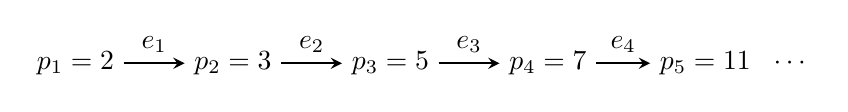
\begin{tikzpicture}[>=stealth,baseline]
\node (a) at (0,0) {$p_1=2$};
\node (b) at (2,0) {$p_2=3$};
\node (c) at (4,0) {$p_3=5$};
\node (d) at (6,0) {$p_4=7$};
\node (e) at (8,0) {$p_5=11$};
\draw[->,thick] (a)--node[above]{$e_1$}(b);
\draw[->,thick] (b)--node[above]{$e_2$}(c);
\draw[->,thick] (c)--node[above]{$e_3$}(d);
\draw[->,thick] (d)--node[above]{$e_4$}(e);
\node at (9.1,0) {$\cdots$};
\end{tikzpicture}
\end{center}

Put \(g_s(x)=\log(1-x^{-s})\), with the branch specified by its
convergent power series for \(x>1\) and \(\Re s>0\).
An elementary discrete-Stokes formula is
\begin{equation}\label{eq:graph-stokes}
 \sum_{n=1}^{N}e_n\bigl(g_s(p_n)-g_s(p_{n+1})\bigr)
 =\sum_{j=1}^{N}(\partial e)_j g_s(p_j)
       -e_Ng_s(p_{N+1}).
\end{equation}
The left side converges absolutely and locally uniformly for \(\Re s>0\).
Indeed, on a compact subset of that half-plane,
\[
 |g'_s(x)|\le C_K x^{-1-\sigma_K}\quad(x\ge2)
\]
for some \(\sigma_K>0\), and
\(\sum_n\int_{p_n}^{p_{n+1}}x^{-1-\sigma_K}\,dx<\infty\).
Since \(g_s(p_n)\to0\), taking \(N\to\infty\) in
\eqref{eq:graph-stokes} gives
\begin{equation}\label{eq:graph-product}
 \boxed{\quad
 \log Q_e(s)
 =\sum_{n\ge1}e_n\bigl[g_s(p_n)-g_s(p_{n+1})\bigr]
 =\sum_{j\ge1}(\partial e)_j g_s(p_j),\quad \Re s>0.
 \quad}
\end{equation}
The second series in \eqref{eq:graph-product} need not be absolutely
convergent: its equality follows from the boundary term in
\eqref{eq:graph-stokes}, not from arbitrary rearrangement.

For \(e_n=1\) on every edge, the interior boundary vanishes and
\(\partial e=(1,0,0,\ldots)\).  Therefore
\[
 \log Q_e(s)=g_s(2),\qquad Q_e(s)=1-2^{-s}.
\]
An infinite occupied ray has only a finite source boundary.  If instead
\(e_n=1\) precisely for \(u\le n\le v\), then
\[
 \partial e=\mathbf 1_{\{u\}}-\mathbf 1_{\{v+1\}},
 \qquad Q_e(s)=\frac{1-p_u^{-s}}{1-p_{v+1}^{-s}}.
\]
For alternating occupied edges, the graph boundary is supported at
every vertex, explaining why cancellation is much weaker.

\subsection{Weighted graph variation and quantitative conditioning}

For a bounded integer-valued edge flow \(h=(h_j)\), let
\begin{equation}\label{eq:graph-TV}
 V_\delta(h):=\sum_{j\ge1}p_j^{-\delta}
                  |h_j-h_{j-1}|,\qquad h_0=0,\quad\delta>0.
\end{equation}
This is the weighted \(\ell^1\)-norm of its incidence boundary,
a discrete bounded-variation quantity on \(G_P\).
For binary perturbations $e,f$, the weighted boundary sum is a sufficient
condition for bounded comparison. It measures transitions in an edge flow,
rather than merely counting moved primes.

\begin{proposition}[Graph-variation stability bound]
\label{prop:graph-conditioning}
Let \(e,f\) be endpoint perturbations and \(0<\delta\le1\).
If \(V_\delta(e-f)<\infty\), then
\(R_{e/f}=Q_e/Q_f\) and its inverse belong to
\(H^\infty(\Re s>\delta)\), and
\begin{equation}\label{eq:graph-stability}
 \max\{\|R_{e/f}\|_\infty,\|R_{e/f}^{-1}\|_\infty\}
 \le \exp\!\left(\frac{V_\delta(e-f)}{1-2^{-\delta}}\right).
\end{equation}
The product of the two operator-multiplier norm bounds is at most
\(\exp(2V_\delta(e-f)/(1-2^{-\delta}))\).
\end{proposition}
\begin{proof}
Put \(h=e-f\), and \(c_j=h_j-h_{j-1}\).
For \(\Re s>\delta\), the estimate
\[
 |\log(1-p_j^{-s})|
 \le \frac{p_j^{-\delta}}{1-p_j^{-\delta}}
 \le \frac{p_j^{-\delta}}{1-2^{-\delta}}
\]
shows that \(\sum_j c_jg_s(p_j)\) converges absolutely and uniformly
and has modulus at most
\(V_\delta(h)/(1-2^{-\delta})\).
Exponentiate \eqref{eq:graph-product} for the quotient, and then
apply the same argument with \(-h\).
\end{proof}

The additive group of bounded integer edge flows contains the subgroup
\(\{h:V_\delta(h)<\infty\}\).
Consequently the binary endpoint perturbations map to equivalence
classes in the quotient by this subgroup.  This is a convenient
graph-cochain description of the arithmetic classification; it does
\emph{not} assert ordinary graph-Laplacian spectral equivalence.

\subsection{A signed-frequency graph for arbitrary interior shifts}

The same bookkeeping works beyond the endpoints.  For a finite
perturbation \(A_N=(a_1,\ldots,a_N)\), draw the oriented edge
\(p_n\to a_n\) on the vertex set of all distinct frequencies
\(\{p_1,\ldots,p_N,a_1,\ldots,a_N\}\).  A loop contributes zero.
The signed vertex boundary is the atomic measure
\[
 \mu_{A,N}:=\sum_{n=1}^N(\delta_{p_n}-\delta_{a_n}).
\]
For every \(\Re s>0\), the finite Euler quotient satisfies
\begin{equation}\label{eq:graph-atomic}
 \log Q_{A,N}(s)=
 \int_{(1,\infty)}\log(1-x^{-s})\,d\mu_{A,N}(x).
\end{equation}
If two edges share a frequency endpoint, their incidence
coefficients may cancel.  Cancellation of this boundary is exact for shared endpoints. A complete
necessary condition for general interior shifts is not asserted.


\subsection{A bounded comparison on the original weighted Sobolev space}

The graph variation also controls the original dilation operators
without first passing to a Hardy-space multiplier representation.
Fix $S_k$ as in Section~\ref{sec:operators}, with
$\alpha=1/(2k)$, and write
$c_j=(e_j-f_j)-(e_{j-1}-f_{j-1})$.

\begin{theorem}[Norm-convergent graph-boundary comparison, new]
\label{thm:graph-Sk}
Suppose that
\begin{equation}\label{eq:graph-Sk-hyp}
 \sum_{j\ge1}|c_j|p_j^{-\alpha}<\infty.
\end{equation}
Then the product
\begin{equation}\label{eq:graph-Sk-operator}
 C_{e/f}=\prod_{j\ge1}(I-R_{p_j})^{c_j}
\end{equation}
converges in operator norm on $S_k$. It has a bounded inverse.
Moreover,
\begin{equation}\label{eq:graph-Sk-bound}
 \max\{\|C_{e/f}\|,\|C_{e/f}^{-1}\|\}
 \le \exp\left(
 \frac{\sum_{j\ge1}|c_j|p_j^{-\alpha}}
 {1-2^{-\alpha}}\right).
\end{equation}
On the algebraic domain $\mathcal D_k$, $C_{e/f}$ is the
multiplier with symbol $\zeta_{A_e}/\zeta_{A_f}$,
where the quotient is understood through its holomorphic
Euler-factor continuation.
\end{theorem}

\begin{proof}
A change of variables in each term of the $S_k$ norm gives
$\|R_p\|\le p^{-\alpha}$. Thus
$\|I-R_p\|\le1+p^{-\alpha}$ and
$\|(I-R_p)^{-1}\|\le(1-p^{-\alpha})^{-1}$.
The logarithms of both bounds are no larger than
$p^{-\alpha}/(1-p^{-\alpha})$.
The hypothesis ensures norm convergence of the products
with exponents $c_j$ and $-c_j$, and gives
\eqref{eq:graph-Sk-bound}. All the factors commute, so the
two products are inverses.
On $y^s$ the symbol is
$\prod_j(1-p_j^{-s})^{c_j}$.
The discrete-Stokes identity \eqref{eq:graph-stokes}
identifies that symbol with the ratio of the two
Euler-product comparisons. On logarithmic powers,
differentiate the normally convergent scalar identity.
\end{proof}

\begin{example}[A fully occupied prime path]
If every prime is moved to the next prime, then
$c_1=1$ and $c_j=0$ for $j>1$ (taking $f_j=0$).
Hence $C_{e/f}=I-R_2$. Infinite arithmetic
perturbations have collapsed to one boundedly invertible
operator factor.
\end{example}

\begin{remark}
This is a sufficient condition for bounded comparison.
It neither proves similarity by conjugation of the full
summation operators nor asserts anything about graph-Laplacian
isospectrality.
\end{remark}

\subsection{The multiplicative graph of generalized integers}

For \(A_N=(a_1,\ldots,a_N)\), consider the graded directed graph
\[
 \Gamma_{A_N}:\quad
 V=\mathbb Z_{\ge0}^{N},\qquad
 \nu\longrightarrow \nu+\mathbf e_j\quad(1\le j\le N).
\]
Give the vertex \(\nu\) the weight
\(w_s(\nu)=\prod_{j=1}^N a_j^{-s\nu_j}\).
Summing \emph{vertices}, rather than all directed paths, gives
\begin{equation}\label{eq:graph-vertexzeta}
 \sum_{\nu\in\mathbb Z_{\ge0}^N}w_s(\nu)
 =\prod_{j=1}^N(1-a_j^{-s})^{-1}
 =\zeta_{A,N}(s),\qquad\Re s>0.
\end{equation}
This vertex interpretation respects the multiplicities of
generalized integers.  For example, \(a_1=a_2=3\) produces
three exponent vectors of total degree two, all evaluating to \(9\);
accordingly the coefficient of \(3^{-2s}\) in
\((1-3^{-s})^{-2}\) is \(3\).  Counting directed paths instead
would introduce different, and incorrect, multiplicities.
The graph in \eqref{eq:graph-vertexzeta} is not an Ihara
nonbacktracking-cycle zeta construction.

\begin{proposition}[Convergent graph-transfer realization]
\label{prop:graph-transfer}
For \(\sigma>1\), let \(X_\sigma\) be the Banach space of functions
on \((0,1]\) with
\[
 \|f\|_{X_\sigma}:=\sup_{0<y\le1}y^{-\sigma}|f(y)|<\infty.
\]
Write \(D_a f(y)=f(y/a)\).  The operator products
\begin{equation}\label{eq:graph-resolvents}
 P_A=\prod_{n\ge1}(I-D_{a_n})^{-1},
 \qquad
 (I-qD_q)P_A\quad(q=2,3)
\end{equation}
converge in operator norm on \(X_\sigma\), and
\begin{equation}\label{eq:graph-literalsum}
 (I-qD_q)P_Af(y)
 =\sum_{m\in\mathcal N_A}
 \left[f(y/m)-qf(y/(qm))\right].
\end{equation}
All sums in \eqref{eq:graph-literalsum} converge absolutely in
\(X_\sigma\).  These operators are boundedly invertible on
\(X_\sigma\).
\end{proposition}
\begin{proof}
The dilation operators commute and
\(\|D_a\|_{X_\sigma}=a^{-\sigma}\).
Since \(a_n\ge p_n\) and
\(\sum_n p_n^{-\sigma}<\infty\), the two products
\(\prod_n(I-D_{a_n})^{-1}\) and
\(\prod_n(I-D_{a_n})\) converge in operator norm and
are inverses.  Expand each geometric series and pass to the
norm limit to obtain the generalized-integer sum with
multiplicity.  Finally,
\(\|qD_q\|=q^{1-\sigma}<1\), so \(I-qD_q\) is invertible
by a Neumann series.
\end{proof}

\begin{remark}[Scope of the graph model]
The space \(X_\sigma\), \(\sigma>1\), is the domain of an
\emph{absolutely convergent} graph-transfer representation.  It
does not contain the zeta-zero eigenfunctions \(y^\rho\) from the
critical strip and is not a substitute for the analytically
continued \(S_k\) operators.  In particular, Proposition
\ref{prop:graph-transfer} proves no kernel invariance in the
critical strip.  It supplies a natural discrete approximation
and separates the convergent graph mechanics from the deeper
operator-domain problem.
\end{remark}

\paragraph{Further graph questions.}
One can ask whether (i) weighted incidence-boundary classes
admit computable finite-section approximations with certified
tails; (ii) equality of closed graph-transfer domains forces
bounded comparison in a natural completion; and (iii) the
graph boundary at infinity controls comparison-operator
conditioning.  These are proposed investigations, not claims
about the spectrum of a graph Laplacian.

\section{Concluding remarks}\label{sec:conclusion}

Three parts of the 1981 program survive. The new graph-theoretic
operator comparison is Theorem~\ref{thm:graph-Sk}.
\begin{enumerate}[label=(\arabic*)]
\item Generator systems close to the primes, in the weighted $\ell^1$
  sense of \eqref{eq:l1}, have the same zeros as $\zeta$.
\item The very regular system $u_n=\Li^{-1}(n)$ has a zero-free zeta
  function, now on a slit half-plane. Comparison with it gives a criterion
  for RH in terms of rare large deviations of $p_n$ from $u_n$.
\item Dilation-sum operators detect zeros through their kernels. With two
  such operators and the generator $\yD$, no parameter $\beta$ is needed.
\end{enumerate}

Two parts do not survive. The block operators $B(\beta)$ have point
spectrum containing $\CC\setminus[0,\infty)$. So their spectra carry no
information about zeros. And the closing hope about pair correlation
remains a motivation only. In particular, the random system of
Section~\ref{sec:random} has no zeros to the right of $\frac12$. So a
random-matrix model of Montgomery's conjecture~\cite{Mo73} would
need a different design. See also Mehta~\cite{Me67}.

\appendix
\section{Glossary}\label{app:glossary}

\begin{description}[style=nextline,leftmargin=1.5em]
\item[Algebraic span] The set of \emph{finite} linear combinations of a
  family of vectors. No limits are taken.
\item[Almost surely] With probability one.
\item[Analytic continuation] Extension of a holomorphic function to a
  larger connected open set. It is unique when it exists.
\item[Beurling generalized primes] Any sequence $1<a_1\le a_2\le\cdots$
  tending to infinity. Formal products of its terms are the generalized
  integers.
\item[Borel--Cantelli lemma] If $\sum\Pr(E_n)<\infty$, then almost surely
  only finitely many events $E_n$ occur.
\item[Branch point] A point around which a function changes value when
  continued around a small loop. Example: $(2s-1)^{-1/2}$ at
  $s=\frac12$.
\item[Closure of an operator] The operator whose graph is the closure of
  the original graph, when that closure is a graph.
\item[Critical strip] The region $0<\Ree s<1$.
\item[Dilation] The map $f(y)\mapsto f(y/c)$.
\item[Dirichlet eta function] $\eta(s)=\sum(-1)^{n-1}n^{-s}$. It equals
  $(1-2^{1-s})\zeta(s)$ and converges for $\Ree s>0$.
\item[Distributional derivative] The derivative in the sense of
  distributions. It agrees with the classical derivative for smooth
  functions.
\item[Incidence boundary] The signed vertex sum of a directed
edge flow; the source is positive and target negative.
\item[Exponent-vector graph] A directed lattice in which
vertices represent formal generalized integers.
\item[Weighted graph variation] The sum of absolute incidence
coefficients weighted by a power of their prime vertices.
\item[Euler product] A product $\prod(1-a_n^{-s})^{-1}$ over generators.
\item[Exponential integral] $E_1(z)=\int_z^\infty e^{-t}\,\dd t/t$. It
  equals $-\gamma-\Log z$ plus an entire function.
\item[Hoeffding's inequality] A tail bound for sums of bounded
  independent random variables.
\item[Joint kernel] The set of vectors killed by each of several
  operators.
\item[Jordan block] A matrix with one eigenvalue on the diagonal and ones
  just above it.
\item[Logarithmic integral] $\Li(x)=\mathrm{P.V.}\int_0^x\dd t/\log t$.
\item[Mellin transform] The transform $f\mapsto\int_0^\infty f(y)y^{s-1}
  \dd y$. It turns dilations into multiplication by $c^{-s}$.
\item[Meromorphic] Holomorphic except for isolated poles.
\item[Multiplier operator] An operator that acts on $y^s$ by a scalar
  $F(s)$, called its symbol.
\item[Nontrivial zero] A zero of $\zeta$ in the critical strip.
\item[Normal convergence] Convergence of $\sum\sup_K|f_n|$ on every
  compact set $K$.
\item[Periodic residue cycle] A directed cycle of residue
classes modulo $q$, with its zero-mean Fourier modes.
\item[Point spectrum] The set of eigenvalues of an operator.
\item[Prime zeta function] $P_A(s)=\sum_na_n^{-s}$.
\item[Resolvent set] The set of $\lambda$ for which $\lambda-M$ has a
  bounded inverse.
\item[Riemann hypothesis (RH)] All nontrivial zeros of $\zeta$ have real
  part $\frac12$.
\item[Spectral synthesis] The property that a closed invariant subspace
  is the closed span of the exponential (or power) functions it contains.
\item[Stieltjes integral] An integral $\int f\dd g$ with respect to a
  function $g$ of bounded variation, such as a counting function.
\item[Weighted Sobolev space] A space of functions whose derivatives up
  to some order are square integrable against given weights.
\end{description}

\section*{Acknowledgments and provenance}
\addcontentsline{toc}{section}{Acknowledgments and provenance}

The 1981 typescript contains the following acknowledgments.
\begin{quote}\itshape
I thank Paul Erd\H{o}s for his inspiration. He has also pointed out that
another random number theoretic approach, comparative to our section~1,
has been initiated by Hawkins. See~[7] for a recent set of references and
summary.

In conclusion, I gratefully acknowledge the encouraging and adroit
suggestions of my teacher Professor Johan Belinfante, who effected many
significant improvements in section~3.
\end{quote}
(The typescript separates some of these clauses with semicolons. We have
split them into sentences.) These acknowledgments do not imply that either
mathematician reviewed the present edition.

The first corrected edition (ChatGPT, 2026) supplied the repaired proofs of
the original Theorems~1--4 and the first counterexample. This second
edition (Claude, 2026) added the comparison principle, the dyadic lemma,
the slit-plane theorem, the triangular-block lemma, the multiplier
calculus and Section~\ref{sec:betafree}. ChatGPT (OpenAI) prepared Draft 3 with new graph constructions,
proofs, editorial changes and compilation checks. Claude (Anthropic)
prepared the second corrected edition. AI review is not an independent
certification of the results. More detail appears in the separate
revision log. All mathematics used here was available in 1981.


\begin{thebibliography}{99}

\bibitem{BD69} P.~T. Bateman and H.~G. Diamond, Asymptotic distribution
of Beurling's generalized prime numbers, in \emph{Studies in Number
Theory}, MAA Studies in Mathematics~6, 1969, 152--210.

\bibitem{Be37} A.~Beurling, Analyse de la loi asymptotique de la
distribution des nombres premiers g\'en\'eralis\'es, \emph{Acta Math.}
\textbf{68} (1937), 255--291.

\bibitem{Be55} A.~Beurling, A closure problem related to the Riemann
zeta-function, \emph{Proc. Nat. Acad. Sci. U.S.A.} \textbf{41} (1955),
312--314.

\bibitem{GS78} E.~Grosswald and F.~J. Schnitzer, A class of modified
$\zeta$ and $L$-functions, \emph{Pacific J. Math.} \textbf{74} (1978),
357--364.

\bibitem{Ha58} D.~Hawkins, The random sieve, \emph{Math. Mag.}
\textbf{31} (1958), 1--3.

\bibitem{He78} C.~C. Heyde, A loglog improvement to the Riemann
hypothesis for the Hawkins random sieve, \emph{Ann. Probab.} \textbf{6}
(1978), 870--875.

\bibitem{Ho63} W.~Hoeffding, Probability inequalities for sums of
bounded random variables, \emph{J. Amer. Statist. Assoc.} \textbf{58}
(1963), 13--30.

\bibitem{In32} A.~E. Ingham, \emph{The Distribution of Prime Numbers},
Cambridge Tracts in Mathematics~30, Cambridge University Press, 1932.

\bibitem{Ko59} D.~D. Kosambi, An application of stochastic
convergence, \emph{J. Indian Soc. Agricultural Statist.} \textbf{11}
(1959), 59--72.

\bibitem{Li14} J.~E. Littlewood, Sur la distribution des nombres
premiers, \emph{C. R. Acad. Sci. Paris} \textbf{158} (1914), 1869--1872.

\bibitem{Me67} M.~L. Mehta, \emph{Random Matrices and the Statistical
Theory of Energy Levels}, Academic Press, New York, 1967.

\bibitem{Mo73} H.~L. Montgomery, The pair correlation of zeros of
the zeta function, in \emph{Analytic Number Theory}, Proc. Sympos. Pure
Math.~24, Amer. Math. Soc., 1973, 181--193.

\bibitem{Ny50} B.~Nyman, \emph{On the One-Dimensional Translation Group
and Semi-Group in Certain Function Spaces}, Thesis, Uppsala, 1950.

\bibitem{Ra38} R.~A. Rankin, The difference between consecutive prime
numbers, \emph{J. London Math. Soc.} \textbf{13} (1938), 242--247.

\bibitem{Sc47} L.~Schwartz, Th\'eorie g\'en\'erale des fonctions
moyenne-p\'eriodiques, \emph{Ann. of Math.} \textbf{48} (1947), 857--929.

\bibitem{Ti51} E.~C. Titchmarsh, \emph{The Theory of the Riemann
Zeta-Function}, Clarendon Press, Oxford, 1951.

\bibitem{vK01} H.~von Koch, Sur la distribution des nombres premiers,
\emph{Acta Math.} \textbf{24} (1901), 159--182.

\bibitem{Wi44} A.~Wintner, \emph{The Theory of Measure in Arithmetical
Semi-Groups}, Waverly Press, Baltimore, 1944.

\bibitem{Wu74} M.~C. Wunderlich, A probabilistic setting for prime
number theory, \emph{Acta Arith.} \textbf{26} (1974), 59--81.

\bibitem{Yo74} K.~Yosida, \emph{Functional Analysis}, 4th ed.,
Springer-Verlag, Berlin, 1974.

\end{thebibliography}
\end{document}
